\chapter{Analysis of the circuit}
\begin{figure}[h]
\centering
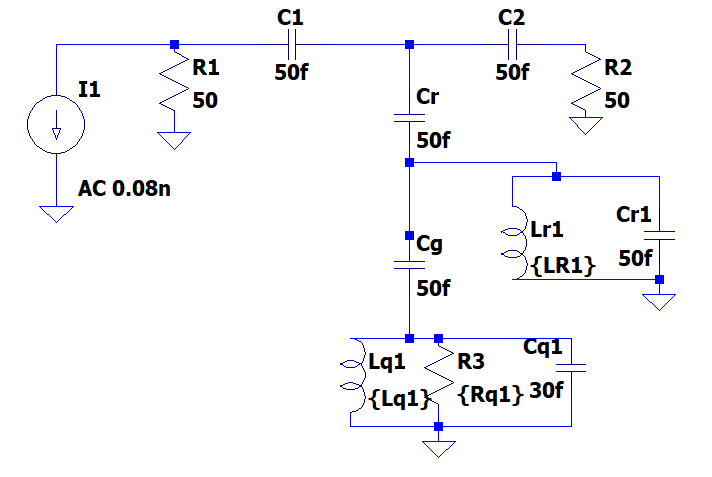
\includegraphics[width=0.7\linewidth, height=0.4\linewidth, keepaspectratio]{./exercise 5/TransmissionLineQubit.png}
\caption{Transmission line coupled to the qubit and readout resonator implemented in LTspice.}
\label{fig:transmission_line_qubit}
\end{figure}

The circuit shown in Fig.~\ref{fig:transmission_line_qubit} is analyzed for three different values of the qubit inductance, namely $L_{q1} = 20.45\,$nH, $23.45\,$nH, and $26.45\,$nH, in order to evaluate its impact on the system response.

\begin{figure}[h]
\centering
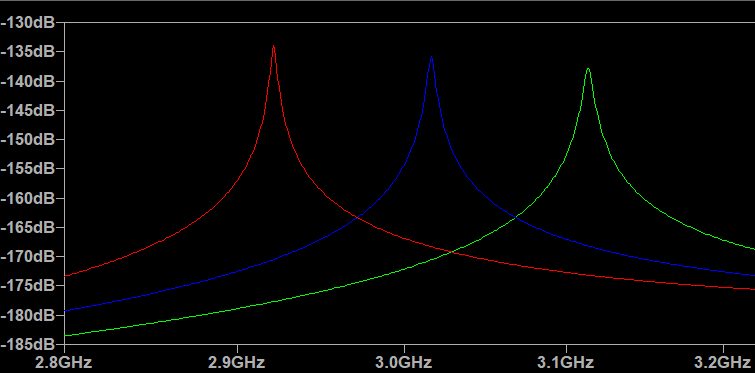
\includegraphics[width=0.8\linewidth]{./exercise 5/ThreePeaks.png}
\caption{Resonance peaks for different values of the qubit inductance.}
\label{fig:three_peaks}
\end{figure}

From the Bode plot in Fig.~\ref{fig:three_peaks}, it is observed that the position of the resonance peak varies with the inductance. This behavior is consistent with the dependence of the resonance frequency on the $LC$ parameters of the qubit, according to

\begin{equation}
f_q = \frac{1}{2\pi\sqrt{L_q C_q}}.
\end{equation}

\needspace{3\baselineskip}
The extracted peak frequencies are reported in the following table:

\begin{table}[H]
\centering
\begin{tabular}{c c}
\hline
Step & $f_{\text{peak}}$ (Hz) \\
\hline
1 & $3.113 \times 10^{9}$ \\
2 & $3.016 \times 10^{9}$ \\
3 & $2.921 \times 10^{9}$ \\
\hline
\end{tabular}
\caption{Peak frequencies for different values of the qubit inductance.}
\end{table}

The results show a clear shift of the resonance frequency as the qubit inductance is modified.

This variation of $L_q$ effectively models the action of the flux line, which tunes the qubit frequency by modifying its effective Josephson inductance, allowing controlled shifts of the resonance.